\chapter{Introducción}

\section{Definiciones introductorias}

\begin{itemize}
	\item \textbf{Procesador}: Sistema cuyo objetivo es el procesamiento de una entrada con el fin de producir una salida.
	\item \textbf{Lenguaje}: Conjunto de cadenas formadas por elementos tomados de un alfabeto.
	\item \textbf{Procesador de lenguajes}: Toma como entrada cadenas de un lenguaje, que son procesadas para producir una salida.
	\item \textbf{Traductor}: Entrada texto en $L_1$ (lenguaje fuente) y salida texto en $L_2$ (lenguaje objeto, preservando el significado).
	\item \textbf{Intérprete}: procesa las instrucciones del lenguaje fuente y las ejecuta, NO las traduce.
\end{itemize}

\begin{figure}[h]
	\centering
	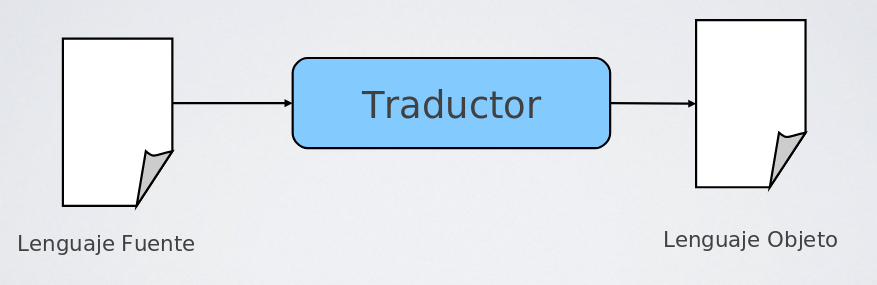
\includegraphics[width=0.7\linewidth]{img/1}
	\caption{}
	\label{fig:1}
\end{figure}

\textbf{Tipos de traductores:}
\begin{center}
	\begin{tabular}{|c|c|c|}
		\hline 
		& \textbf{Lenguaje fuente (L1)} & \textbf{Lenguaje objeto (L2)}  \\ 
		\hline 
		Compilador & Lenguaje alto nivel & Lenguaje máquina  \\ 
		\hline 
		Ensamblador & Lenguaje ensamblador & Lenguaje máquina  \\ 
		\hline 
		Preprocesador & L. Alto nivel con extensiones & L. Alto Nivel sin extensiones \\ 
		\hline 
		Conversor fuente-fuente & Lenguaje de Alto nivel & Lenguaje de Alto nivel (distinto)  \\ 
		\hline 
		Decompilador & Lenguaje de Bajo nivel & lenguaje de Alto nivel \\ 
		\hline 
	\end{tabular} 
\end{center}

\section{Lenguajes, gramáticas y autómatas}
\textbf{¿Qué es una gramática?}\newline
Las gramáticas son un ente formal para especificar de manera finita, el conjunto de cadena de símbolos potencialmente infinitos que constituyen un lenguaje.
Una gramática es una cuádrupla(V,T,P,S):
\begin{itemize}
	\item V: símbolos no terminales.
	\item T: símbolos terminales.
	\item P: reglas de producción.
	\item S: símbolo inicial de la gramática.
\end{itemize}
Podemos definir las cadenas que pertenecen al lenguaje por \textbf{extensión} o por \textbf{derivación} (a partir de su gramática y símbolo inicial). Existen varios tipos de gramáticas:
\begin{itemize}
	\item \textbf{Gramática tipo 0}: Sin restricciones o de estructuras de frases.
	\item \textbf{Gramática tipo 1}: Sensibles al contexto.
	\item \textbf{Gramática tipo 2}: Independientes del contexto.
	\item \textbf{Gramática tipo 3}: Regulares.
\end{itemize}
\begin{figure}[h]
	\centering
	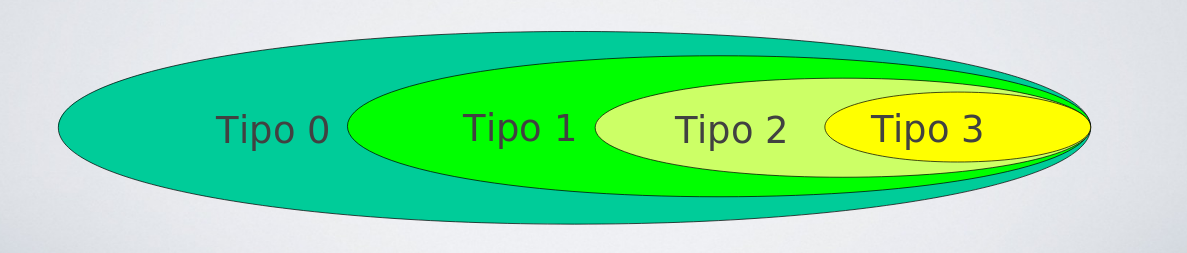
\includegraphics[width=0.5\linewidth]{img/2}
	\caption{}
	\label{fig:2}
\end{figure}

El lenguaje generado por una gramática G=(V,T,P,S), será notado como L(G), y se define como el conjunto de cadenas formadas por símbolos terminales que son derivables a partir del símbolo inicial de la gramática.

\begin{center}
	$L(G)=\{u\epsilon T | S \Rightarrow u\}$
\end{center}

\begin{center}
	\begin{tabular}{|c|c|c|}
		\hline 
		Gramáticas	& Lenguajes  & Máquinas \\ 
		\hline 
		GLC & Libre de contexto & Autómatas a Pila \\ 
		\hline 
		GR & Regular & Autómatas Finitos\\ 
		\hline 
	\end{tabular} 
\end{center}

\section{Derivación de una gramática}
Dada una gramática G(V,T,P,S) y dos palabras $\alpha$,$\beta \epsilon$ (V$\cup$T)$\ast$, solo decimos que $\beta$ es derivable a partir de $\alpha$ en un paso ($\alpha \Rightarrow \beta$) si y solo si existen palabras $\delta_1, \delta_2 \epsilon$ (V$\cup$T)$\ast$ y una producción Y $\longrightarrow \emptyset$ tales que $\alpha = \delta_1$ y $\delta_2$ y $\beta$= $\delta_1 \emptyset \delta_2$
\section{Definición de un lenguaje}
La definición de un lenguaje implica:
\newline
\newline
\textbf{Léxico}: vocabulario del lenguaje junto con sus categorías. Por ejemplo, en un lenguaje de programación, dentro de la categoría tipos, podríamos encontrar el vocabulario (int, float,double, etc).
\newline
\newline
\textbf{Sintáctico}: Reglas que establecen como construir frases válidas del lenguaje usando los elementos del vocabulario.
\newline
\newline
\textbf{Semántico}: El significado de las frases, es la información de la cadena, por ejemplo al leer la cadena, "int v = 0", el significado es "una variable numérica v se asigna el valor 0".
\newline
\newline
El léxico corresponde a un lenguaje regular, por lo que se expresa con una GR. Por otro lado, el sintáctico se corresponde con una GLC (aunque no tiene por qué ser al completo).
\newline
\newline
Para distinguir una GR de un GLC hay que fijarse en la parte derecha de la producción y ver si tiene uno o mas no terminales.

\section{Estructura de un traductor}
El proceso de la traducción implica dos fases:
\begin{itemize}
	\item \textbf{Fase de Análisis}(front end): Comprueba que el texto de entrada esta escrito conforme a las reglas (léxicas y sintácticas del lenguaje). Esta fase es dependiente del lenguaje.
	\item \textbf{Fase de Síntesis} (back end): Genera texto equivalente optimizado en el lenguaje objeto. Esta fase es dependiente de la máquina.
\end{itemize}

\begin{figure}[h]
	\centering
	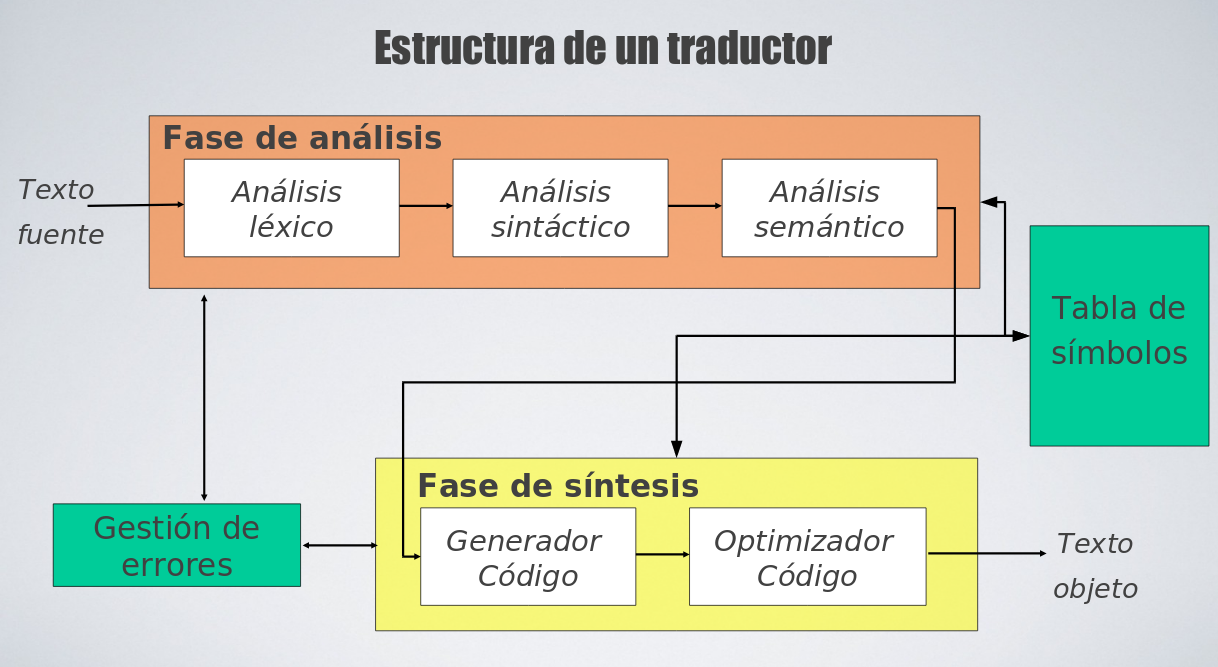
\includegraphics[width=0.7\linewidth]{img/4}
	\caption{}
	\label{fig:4}
\end{figure}

En el análisis léxico se va iterando carácter a carácter, reconociendo si son palabras válidas del lenguaje. Es decir lee
la palabra “int” y deduce la categoría “tipos”. Elimina e ignora espacios, tabuladores, saltos de línea, etc. Después en
el análisis sintáctico se leen las palabras recibidas (una vez de sabe que pertenecen al lenguaje), y se itera desde el
símbolo inicial de la gramática esa secuencia de palabras, así se comprueba que la estructura es correcta. Finalmente,
en el análisis semántico se recibe “el árbol de derivación” (o un equivalente) y se determina que función hace esa
cadena introducida. Cuando sabe su funcionamiento, lo transmite al generador de código, para que el lenguaje objeto
tenga la misma función.

\section{Técnicas de construcción de traductores con T-Diagramas}
Una notación muy útil para describir programas en general y traductores en particular, son los llamados T-Diagramas.
\begin{figure}[h]
	\centering
	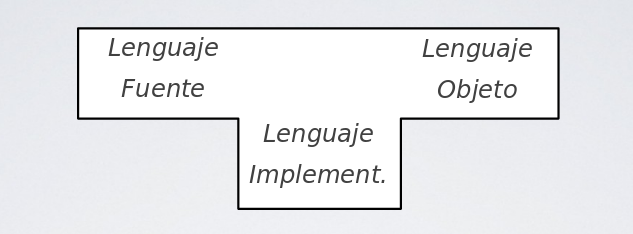
\includegraphics[width=0.7\linewidth]{img/5}
	\caption{}
	\label{fig:5}
\end{figure}


En el siguiente diagrama tipo T se explica el funcionamiento del procesador que se pretende implementar, tomamos \textbf{ Mor } como lenguaje fuente, y Java como lenguaje objeto, y además el lenguaje que implementa es Java, es decir, nuestro compilador compila a Java, y esta escrito a Java. 
\newline
\newline
Para utilizar ese compilador, utilizamos un compilador auxiliar, que está escrito en código máquina para dar lugar a bytecode, el típico archivo \textbf{.class} que generamos al compilar un \textbf{.java}.
\newline

Por último tenemos que compilar el bytecode, con un compilador que acepta bytecode escrito en código máquina.
\begin{figure}[h]
	\centering
	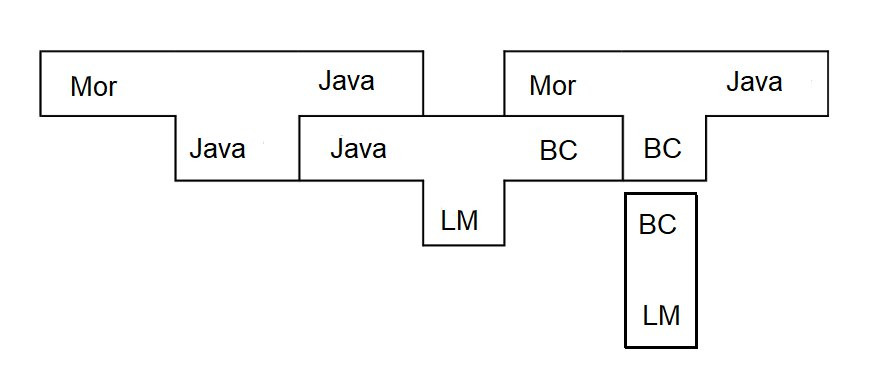
\includegraphics[width=0.7\linewidth]{img/photo5978652419892031524}
	\caption{}
	\label{fig:photo5978652419892031524}
\end{figure}



